\documentclass[final]{beamer}
\usepackage[size=custom,width=121.92,height=91.44,scale=1.12]{beamerposter}

\usetheme{default}
\usecolortheme{default}
\beamertemplatenavigationsymbolsempty

\usepackage[T1]{fontenc}
\usepackage[utf8]{inputenc}
\usepackage{amsmath,amssymb,amsfonts,mathtools}
\usepackage{booktabs}
\usepackage{array}
\usepackage{graphicx}
\usepackage{ragged2e}
\usepackage{lmodern}
\usepackage{microtype}

\definecolor{PosterPaper}{HTML}{F7F5F0}
\definecolor{PosterInk}{HTML}{182033}
\definecolor{PosterMuted}{HTML}{667085}
\definecolor{PosterGrid}{HTML}{D4DBE6}
\definecolor{PosterBlue}{HTML}{3658C7}
\definecolor{PosterTeal}{HTML}{0D776A}
\definecolor{PosterViolet}{HTML}{6E53E9}
\definecolor{PosterOchre}{HTML}{BF911F}
\definecolor{PosterRust}{HTML}{B85C2E}
\definecolor{PosterGray}{HTML}{9199A8}
\definecolor{PosterPanel}{HTML}{FFFFFF}
\definecolor{PosterSoft}{HTML}{EDF1F7}

\setbeamercolor{background canvas}{bg=PosterPaper}
\setbeamercolor{normal text}{fg=PosterInk,bg=PosterPaper}
\setbeamercolor{title in headline}{fg=white,bg=PosterInk}
\setbeamercolor{author in headline}{fg=white,bg=PosterInk}
\setbeamercolor{institute in headline}{fg=white,bg=PosterInk}
\setbeamercolor{block title}{fg=white,bg=PosterInk}
\setbeamercolor{block body}{fg=PosterInk,bg=PosterPanel}
\setbeamercolor{block title alerted}{fg=white,bg=PosterTeal}
\setbeamercolor{block body alerted}{fg=PosterInk,bg=PosterPanel}
\setbeamercolor{block title example}{fg=white,bg=PosterBlue}
\setbeamercolor{block body example}{fg=PosterInk,bg=PosterPanel}

\setbeamerfont{title}{series=\bfseries,size=\VeryHuge}
\setbeamerfont{author}{series=\bfseries,size=\large}
\setbeamerfont{institute}{size=\normalsize}
\setbeamerfont{block title}{series=\bfseries,size=\Large}
\setbeamerfont{block body}{size=\normalsize}

\setlength{\parskip}{0.35em}
\setlength{\leftmargini}{1.2em}

\newcommand{\RR}{\mathbb{R}}
\newcommand{\EE}{\mathbb{E}}
\newcommand{\one}{\mathbf{1}}
\newcommand{\cA}{\mathcal{A}}
\newcommand{\simplex}{\Delta}
\newcommand{\norm}[1]{\left\lVert #1 \right\rVert}
\newcommand{\inner}[2]{\left\langle #1, #2 \right\rangle}
\newcommand{\paren}[1]{\left( #1 \right)}
\newcommand{\braces}[1]{\left\{ #1 \right\}}
\newcommand{\data}[1]{{\rmfamily\textsc{#1}}}
\newcommand{\methodsc}[1]{\ifmmode\text{{\rmfamily\textsc{#1}}}\else{\rmfamily\textsc{#1}}\fi}
\newcommand{\cda}{\methodsc{CDA}}
\newcommand{\vsc}{\methodsc{VSC}}
\newcommand{\piv}{\methodsc{CDA-Piv}}
\newcommand{\bd}{\methodsc{CDA-BD}}
\newcommand{\swad}{\methodsc{SWAD}}
\newcommand{\diwa}{\methodsc{DiWA}}
\newcommand{\eoa}{\methodsc{EoA}}
\newcommand{\erm}{\methodsc{ERM}}

\title{CDA: Post-hoc Domain Generalization by Distributional Canalization}
\author{Jayden Jeong \and Vijayan K. Asari}
\institute{MSTC, Paul Laurence Dunbar High School \and University of Dayton Vision Lab}

\begin{document}
\begin{frame}[t]
\begin{beamercolorbox}[wd=\paperwidth,sep=1.2cm,leftskip=1.0cm,rightskip=1.0cm]{title in headline}
    {\usebeamerfont{title}\inserttitle\par}
    \vspace{0.35cm}
    {\usebeamerfont{author}\insertauthor\par}
    \vspace{0.15cm}
    {\usebeamerfont{institute}\insertinstitute\par}
    \vspace{0.12cm}
    {\normalsize \texttt{jayden.w.jeong@gmail.com} \hfill \texttt{vasari1@udayton.edu}\par}
    \vspace{0.18cm}
    {\normalsize \textbf{Setting:} source-only post-hoc domain generalization. The training run is fixed, a checkpoint bank already exists, and deployment must choose a retained family and averaging weights without target labels.}
\end{beamercolorbox}

\vspace{0.55cm}

\begin{columns}[t,totalwidth=\textwidth]

\begin{column}{0.32\textwidth}

\begin{block}{Problem and Motivation}
\justifying
Domain generalization asks a model to learn from labeled source domains and generalize to an unseen target domain without target labels. In the post-hoc setting, the practical question is narrower and cleaner:
\[
\text{Given a checkpoint bank } \mathcal{B}=\{\theta_1,\ldots,\theta_K\},
\text{ which checkpoints should we average, and why?}
\]

\textbf{Why existing post-hoc rules are incomplete}
\begin{itemize}
\item Uniform late-window soups trust temporal adjacency.
\item \swad{} explains gains through flatter averaged solutions.
\item \diwa{} and \eoa{} explain gains through diversity and ensemble-style selection.
\item None of these directly measures how fragile the deployed model is to \emph{source-mixture shift}.
\end{itemize}

\textbf{CDA thesis}
\begin{itemize}
\item The deployment object should have low source fit, low source-mixture sensitivity, and low soup mismatch.
\item We call this deployment principle \emph{distributional canalization}.
\end{itemize}
\end{block}

\begin{exampleblock}{Target-Risk Certificate}
\justifying
Let the source-domain loss vector be
\[
L(\theta)=\paren{L_1(\theta),\ldots,L_E(\theta)}^\top \in \RR^E,
\qquad
\bar L(\theta)=\frac{1}{E}\one^\top L(\theta),
\]
and let
\[
P_\perp = I-\frac{1}{E}\one\one^\top
\]
project onto the zero-sum subspace.

Under a local source-supported hidden-shift assumption, the target loss satisfies
\[
L_T(\theta)
\le
\bar L(\theta)
+
\rho \norm{P_\perp L(\theta)}_2
+
\epsilon_{\rm app}.
\]

\textbf{Interpretation}
\begin{itemize}
\item \(\bar L(\theta)\): average source fit
\item \(\norm{P_\perp L(\theta)}_2\): sensitivity to redistributing source-domain mass
\item \(\epsilon_{\rm app}\): approximation gap of the local hidden-shift model
\end{itemize}

For soups, a mergeability term bridges endpoint-domain quantities to the deployed averaged model:
\[
L_T(\bar\theta(w))
\le
\bar z(w)
\!+\!
\rho \norm{P_\perp z(w)}_2
\!+\!
\paren{E^{-1/2}+\rho}M(w)
\!+\!
\epsilon_{\rm app}.
\]
\end{exampleblock}

\end{column}

\begin{column}{0.32\textwidth}

\begin{alertblock}{CDA Pipeline}
\justifying
\textbf{Step 1: Version-space compression.}
For each source-support example \((x_i,y_i)\), CDA tracks whether the checkpoint bank disagrees about the true-class confidence threshold:
{\small
\[
D_{\mathcal{B}}(i;\gamma)
=
\mathbf{1}\braces{
\exists j: q_{j,i}\ge \gamma
\ \text{and}\
\exists j': q_{j',i}<\gamma }.
\]
\[
d_{\rm vsc}(S,\mathcal{B};\gamma)
=
\frac{1}{m}\sum_{i=1}^{m}
\mathbf{1}\braces{D_S(i;\gamma)\neq D_{\mathcal{B}}(i;\gamma)}.
\]
}
This keeps a \textbf{non-contiguous} checkpoint family only when it still preserves the source-support disagreement structure that matters for deployment.

\textbf{Step 2: Weight the retained family.}
\begin{itemize}
\item \piv{}: use leave-one-out pivotality, but guard against checkpoints with high source-mixture sensitivity.
\item \bd{}: solve a simplex projection problem toward a balanced low-loss source target set.
\end{itemize}

\textbf{Step 3: Deploy one soup.}
The final model is
\[
\bar\theta(w)=\sum_{j=1}^{k} w_j \theta_j .
\]
\end{alertblock}

\begin{block}{Retained-Family Selection}
\centering
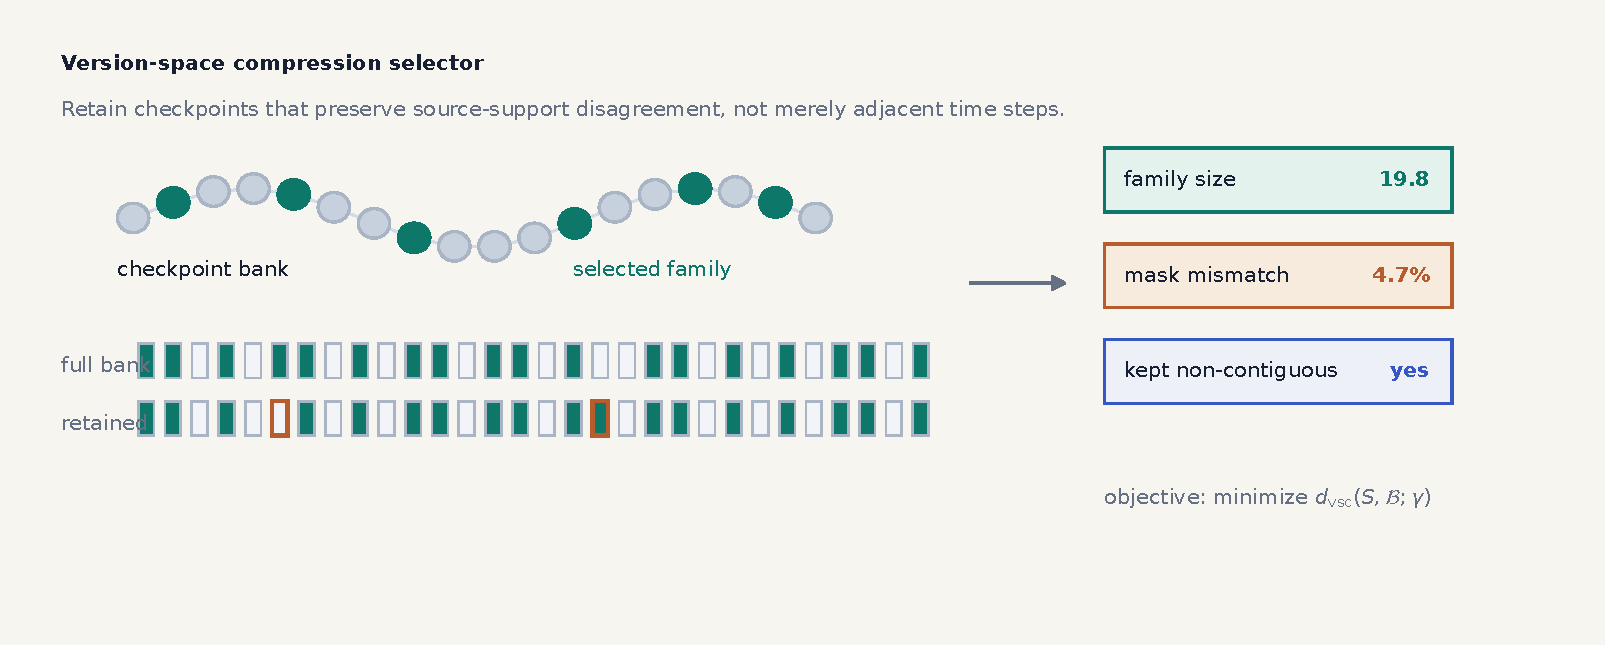
\includegraphics[width=0.98\linewidth]{../figures/vsc_mechanism.pdf}
\end{block}

\begin{block}{Weighting Rules}
\centering
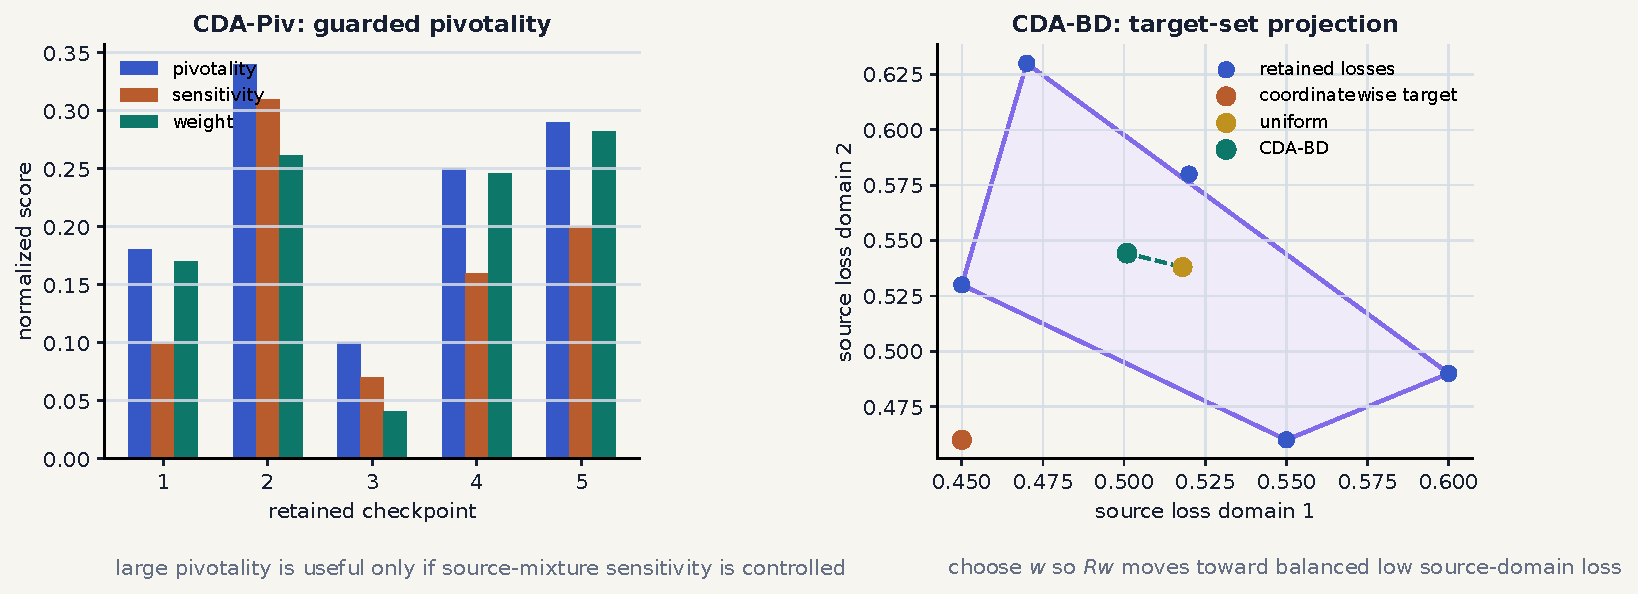
\includegraphics[width=0.98\linewidth]{../figures/weighting_mechanism.pdf}
\end{block}

\end{column}

\begin{column}{0.32\textwidth}

\begin{alertblock}{Headline Results}
\justifying
Across the five-benchmark comparison package, \cda{} reaches
\[
68.3
\]
average OOD accuracy, compared with
\[
66.9 \text{ for } \swad{},
\qquad
68.0 \text{ for } \diwa{},
\qquad
63.3 \text{ for } \erm{}.
\]

\textbf{Real headline reading}
\begin{itemize}
\item \(+5.0\) over ERM on the five-benchmark average
\item \(+1.4\) over SWAD on the five-benchmark average
\item \(+0.3\) over DiWA on the five-benchmark average
\end{itemize}

\centering
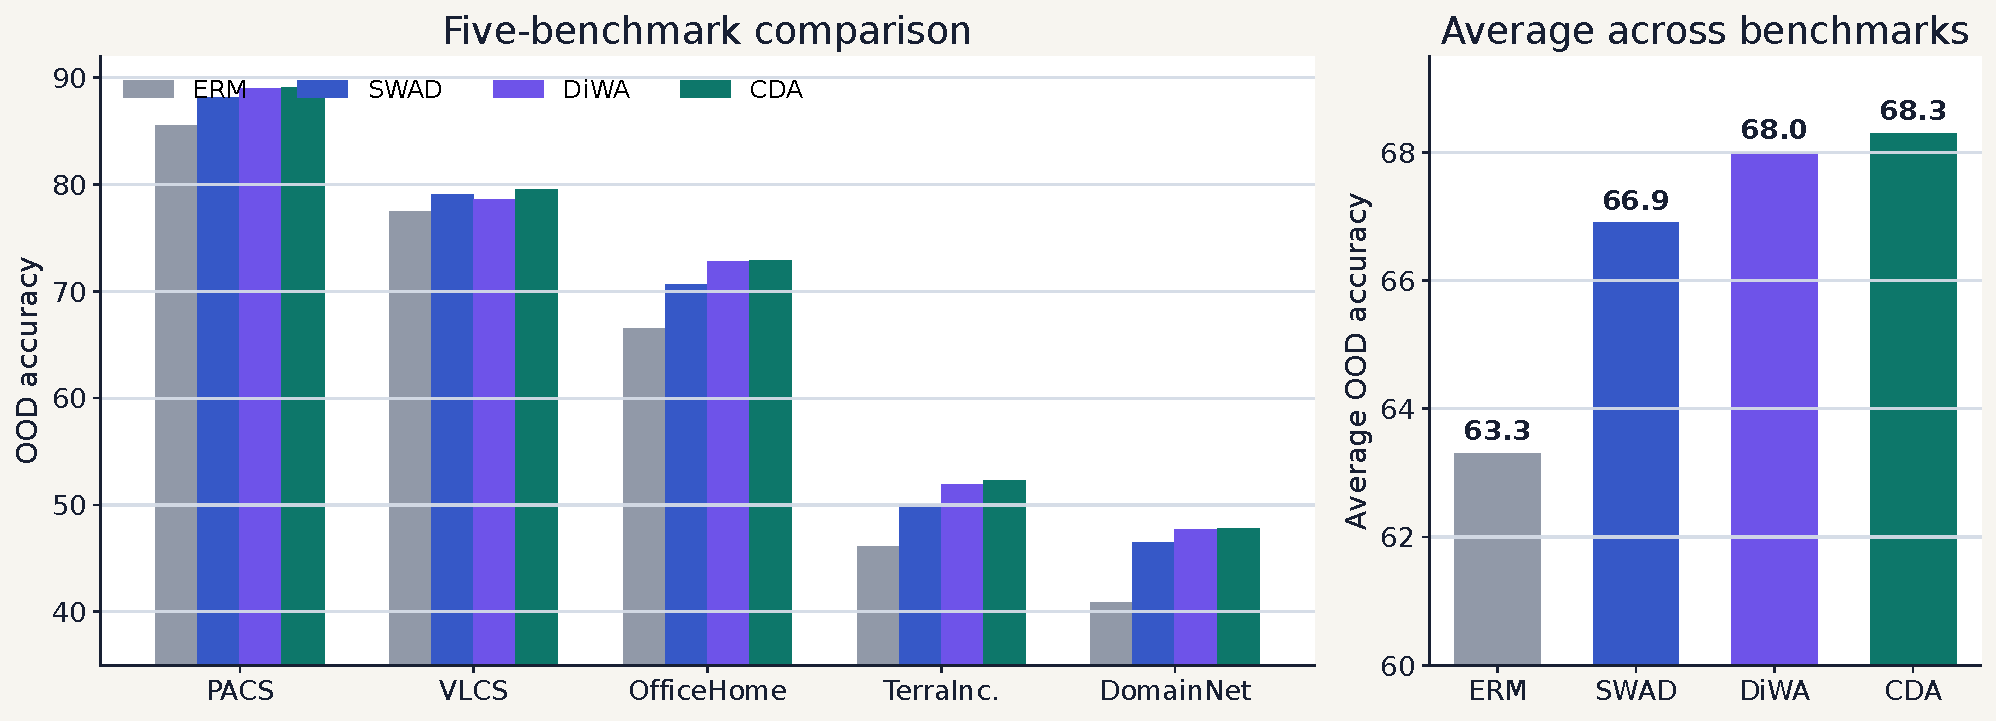
\includegraphics[width=0.98\linewidth]{figures/core_benchmark_results.pdf}
\end{alertblock}

\begin{block}{PACS SWAD-Style Comparison}
\justifying
On the \data{PACS} comparison aligned with the SWAD reporting format, \cda{} reaches:
\[
89.1 \text{ OOD accuracy}
\qquad\text{and}\qquad
97.9 \text{ in-domain accuracy}.
\]
That improves the SWAD OOD number from \(87.1\) to \(89.1\) and the in-domain number from \(97.7\) to \(97.9\).

\centering
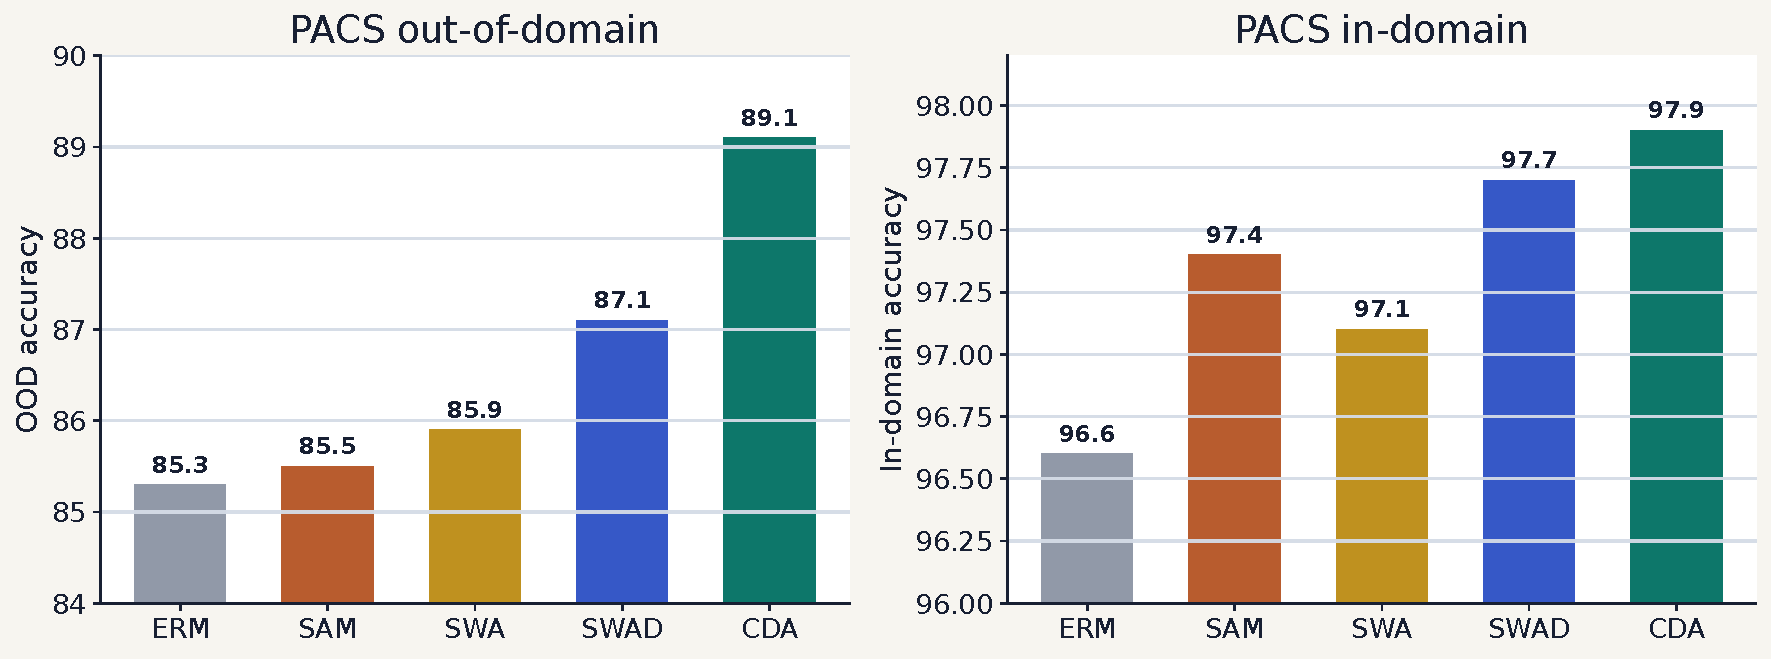
\includegraphics[width=0.98\linewidth]{figures/pacs_generalization.pdf}
\end{block}

\begin{exampleblock}{Takeaways}
\justifying
\begin{enumerate}
\item \textbf{Post-hoc DG can be principled.} The deployment choice can be governed by a source-only certificate rather than by time or heuristic averaging alone.
\item \textbf{Selection matters first.} The retained family must preserve the disagreement structure of the full checkpoint bank.
\item \textbf{Weighting matters second.} Once a good family is retained, CDA turns that structure into a better deployment decision through source-mixture-aware weighting.
\item \textbf{Averaging only helps when the soup is mergeable.} Flatness and local smoothness explain when endpoint-domain quantities transfer to the deployed average.
\end{enumerate}
\end{exampleblock}

\begin{block}{Limitations and Scope}
\justifying
\begin{itemize}
\item CDA studies a \textbf{post-hoc deployment problem}, not the full space of training-time DG algorithms.
\item The theory assumes a \textbf{local source-supported hidden-shift model}. If the target lies far outside nearby source-mixture redistributions, the certificate can loosen.
\item The strongest empirical support on this poster comes from the \textbf{settled benchmark tables} shown here.
\end{itemize}
\end{block}

\end{column}
\end{columns}
\end{frame}
\end{document}
